\chapter{Machine Learning Techniques  to predict CUDA kernels} \label{Chap:ML}

\lettrine[findent=2pt]{\textbf{T}}{}he methods developed in the area of \textbf{big data} (especially machine learning) can be used to predict running times of GPU applications. Information about profiling and traces of heterogeneous parallel applications can be used to improve current Job Managment Systems, which require a better knowledge about the applications~\citep{JMR:Ruiz:2014}. To predict execution times in heterogeneous applications is a great challenge, for this reason, it always is meritorious to research more effective mechanisms to obtain a better performance prediction. Machine learning techniques can learn to capture these interactions without manual intervention, but may require large training sets. 

In this chapter, we compare three different machine learning approaches: linear regression, support vector machines and random forests with a BSP-based analytical model, to predict the execution time of GPU applications. Comparison between these two approaches will be presented using the Mean Average Percentage Error (MAPE). Two different methodologies with machine learning techniques were followed, first a fair comparison is done using the same parameters than analytical model, and second a step of features extraction was performed. In this second process a correlation analysis and hierarchical clustering is done. Profile information was collected of each application over each GPU to use as data input for those ML algorithms.

The rest of this chapter is organized as follows. In Section~\ref{sec:backgroundML} we present background concepts on machine learning techniques and feature extraction. In Section~\ref{sec:method-ML} we describe our experiments and methodology. Section~\ref{sec:resultML} presents the experimental results. Finally, in Section~\ref{sec:relatedWorksML} we review the related works about performance prediction using machine learning techniques.


\section{Concepts and Background}\label{sec:backgroundML}
Machine learning refers to a set of techniques for understanding data. The theoretical subject of ``learning'' is related to prediction. Machine learning techniques involve building a statistical model for predicting, or estimating an output based on one or more inputs. Regression models are used when the output is a continuous value. In this work, we used three different machine learning methods: Linear Regression, Support Vector Machines and Random Forest. There exists other machine learning techniques with sophisticated learning process. However, in this work, we wanted to use simple models to prove that they achieve reasonable predictions.

\subsection{Linear Regression (LR)}
Linear regression is a straightforward technique for predicting a quantitative response $Y$ on the basis of a single or multiple predictor variables $X_p$. It assumes that there is approximately a linear relationship between each $X_p$ and $Y$. It gives to each predictor a separate slope coefficient in a single model. Mathematically, we can write the multiple linear regression model as
\begin{equation}
Y \approx \beta_0 + \beta_1 X_1 + + \beta_2 X_2 + \ldots + + \beta_p X_p + \epsilon
\end{equation}
where $X_p$ represents the $p$th predictor and $\beta_p$ quantifies the association between that variable and the response.

\subsection{Support Vector Machines (SVM)}
Support Vector Machines is a widely used technique for classification and regression problems. It belongs to the general category of kernel methods, which are algorithms that depend on the data only through dot-products. The dot product can be replaced by a kernel function which computes a dot product in some possibly high dimensional feature space $Z$. It maps the input vector $x$ into the feature space $Z$ though some nonlinear mapping. 

\subsection{Random Forest (RF)}
Random Forests belong to decision tree methods, capable of performing both regression and classification tasks. In general, a decision tree with $M$ leaves divides the feature space into $M$ regions $R_m$, $1 \leq m \leq M$. The prediction function of a tree is then defined as $f(x) = \sum_{m=1}^{M} c_m I(x, R_m)$, where $M$ is the number of leaves in the tree, $R_m$ is a region in the features space, $c_m$ is a constant corresponding to region $m$ and $I$ is the indicator function, which is 1 if $x \in R_m$, 0 otherwise. The values of $c_m$ are determined in the training process. Random forest consists of an ensemble of decision trees and uses the mode of the decisions of individual trees.

\subsection{Extraction Features Techniques}\label{ssec:ML}

Correlation techniques and hierarchical clustering algorithm were used in the phase of extraction features to reduce dimensionality of the features. Here, we show a short theoretical background of the techniques used in this work. 

There exist different correlation functions, among them, Pearson, Spearman and Kendal. The Pearson's correlation evaluates the linear relationship between two continuous variables, but omit variation in different scales. The Spearman's correlation evaluates the monotonic relationship between two continuous or ordinal variables. Besides Spearman correlation consider relations in different scales and spaces of the features due to the rank variables.

Pearson's correlation is commonly represented by the greek letter ($\rho$) when it is used for populations and by the letter $r$ when it is used for samples. We will denote it with the letter $r$, the formula for $r$ in a simplified form is
\begin{equation}
r=\frac{\text{cov}(X,Y)}{\sigma_{X}\sigma_{Y}},
\end{equation}
where, cov($X,Y$) is the covariance between two variables, $X$ and $Y$, $\sigma_{X}$ is the standard deviation of $X$ and $\sigma _{Y}$ is the standard deviation of $Y$.

The Spearman correlation coefficient is defined as the Pearson correlation coefficient between the ranked variables~\citep{myers2010research}, for a sample of size $n$, the $n$ raw scores $X_{i}$, $Y_{i}$ are converted to ranks rg$X_{i}$ rg$Y_{i}$. Here, this correlation is denoted as $r_s$, the formula for $r_s$ in a short manner is
\begin{equation}
r_{s}=\frac{\text{cov}(rgX,rgY)}{\sigma_{rgX}\sigma_{rgY}},
\end{equation}
where cov($rgX,rgY$) is the covariance of the rank variables, and $\sigma_{rgX}$ and $\sigma_{rgY}$ are the standard deviations of the rank variables. 

Hierarchical clustering creates groups from a distance matrix. Different metrics or distance functions exist in the literature, among them, Euclidean, Manhattan, Canberra, Binary or Minkowski, however, correlation functions can be also used. A heatmap of pair-wise correlations is a simple way to discover relationships between  pairs of quantitative variables in a dataset. A dendrogram is a tree diagram frequently used to illustrate the arrangement of the clusters produced by a hierarchical clustering algorithm. In Figure \ref{fig:heatMaphClust} is shown a dendrogram with its respective distance matrix using a Spearman correlation function. We can see in this figure a dendrogram with 10 different features about the profile information. In this figure red cells have a high correlation while blue cells have a low correlation.

\begin{figure}[htpb]
    \centering
    \includegraphics[scale=.5]{./images/heatMap.pdf}
    \caption{Heatmap and Dendrogram of a correlation matrix with some features in the experiments}
    \label{fig:heatMaphClust}
\end{figure}

A dendrogram is a tree diagram frequently used to illustrate the arrangement of the clusters produced by hierarchical clustering algorithms. In Figure \ref{fig:heatMaphClust} is shown a dendrogram with its respective matrix of correlation. This dendrogram can be cut in a certain height to permit create a specific number of clusters.

\section{Methodology}\label{sec:method-ML}
This section presents the experiments done with machine learning techniques to predict GPU kernels. Two different approaches with machine learning were proposed. First approach was done with the same features than analytical model, trying to be fair with the analytical model; and second approach was done using a phase of features extraction. 

The methodology of the first approach is shown in Section~\ref{ssec:methodFair} and the methodology of the second approach is presented in Section~\ref{ssec:methodExrtact}. 
In the second approach was used correlation analysis and hierarchical clustering to select the features to use a input in the machine learning algorithms. Profile information was collected of each Application over each GPU. 
We used three different machine learning methods: Linear Regression, Support Vector Machines and Random Forest. 
There exists other machine learning techniques with sophisticated learning process. However, in this work, we wanted to use simple models to prove that they achieve reasonable predictions.

The error of the predictions is presented using the Mean Absolute Percentage Error (MAPE), see equation~\ref{ec:MAPE}. In this equation, $t_m$ is the measured time and $t_k$ is the predicted time. With this error we have analysed the reliability of our approaches. 

\begin{equation}
    mape = \frac{100}{n}\sum _{t=1}^{n}\left|{\frac {{t_m}-{t_k}}{{t_m}}}\right| \label{ec:MAPE}
\end{equation}

We used R to automate the statistical analyses, in conjunction with the \texttt{e1071} and \texttt{randomForest} packages to use the \texttt{svm} and \texttt{randomForest} functions respectively. Collected data, experimental results and source codes are publicly available\footnote{Hosted at GitHub: \texttt{\scriptsize https://github.com/marcosamaris/gpuperfpredict} [Accessed on 6 march 2018]} under Creative Commons Public License. 

To perform our experiments with machine learning techniques, we first collected the performance profiles (metrics and events) for each kernel and GPU. 
All data was collected using the CUDA profiling tool \textbf{nvprof}. This profiling tool enables us to collect data from the command-line reducing the overhead of this process. This process is done without modifications on application source codes. nvprof has four modes to collect information from command-line: summary mode, GPU-trace/API-trace mode, event/metric summary mode and event/metric trace mode. We have used GPU-trace mode and event/metric trace mode.

GPU-trace mode permits collecting data only from CUDA API functions, such as kernel executions, memory transfer throughput between CPU and GPU, among others, without the overhead of profiling the main instructions. Execution times were collected in this mode, along with other features, such as CUDA grid and block dimensions, number of registers per thread, static and dynamic shared memory, device information, streams and the name of executed kernels. A total of 16 features were collected in this mode. 

In event/metric trace mode, all events and metrics are collected for each kernel execution. Although this causes a large overhead in the execution of the kernels, it gives detailed information about the behavior and performance of the executed CUDA kernel functions. All applications were iterated over their selected parameters. The number of events and metrics varied according to the compute capability of the GPUs. All collected information resulted in an approximated size of 12.5GB and the process spent up to 14 days in each GPU. 

For each sample, the metrics, events and traces information were collected in different phases, therefore avoiding the overhead over the measured execution time of the application. The execution time was taken from GPU-trace mode, thus each GPU-trace was executed ten times, and for the experiments was taken the mean of these samples and it was with a confidence interval of 95\%. 


\subsection{Machine Learning without extraction features}\label{ssec:methodFair}
These experiments were done with all the kernels presented in Section~\ref{ssec:useCases}, we used the two-dimensional applications (matrix multiplication and matrix addition) using three different sizes for the CUDA thread blocks, $8^2$, $16^2$ and $32^2$, and input sizes or matrix sizes we vary from $2^{8}$ to $2^{13}$ increasing the matrix size in a step of $2^8$. We took 32 samples per block size, resulting in 96 samples per GPU and a total of 768 samples. For the uni-dimensional problems (dot product and vector addition), the number of thread blocks also was varied in three configurations, $8^2$, $16^2$ and $32^2$, and we used input sizes or vector sizes from $2^{17}$ to $2^{28}$. From $2^{17}$ to $2^{22}$ 6 samples were taken, and from $2^{23}$ to $2^{28}$ 63 samples were taken. For these two applications 69 samples for each configuration were taken, resulting in 207 samples per GPU and a total of 1656 samples. For sub-array maximum problem, 69 samples with the original configuration were taken, for a total of 552 samples. 

All Rodinia applications were iterated over their selected parameters shown in Table~\ref{tab:GPUs}. For most kernels of Rodinia applications, we generated many samples, but we could generate only 57 samples on each GPU from the Back-Propagation (BCK) application. To limit the bias on the learning algorithms, we selected 100 random samples from the other applications in both approaches. It was, this sampled data, that was used as dataset for the ML algorithms in both approaches. 

To be fair with the analytical model, we then choose similar communication and computation parameters to use as feature inputs for the machine learning algorithms. We performed the evaluation using cross-validation, that is, for each target GPU, we performed the training using the other 8 GPUs, testing the model in the target GPU. This process was done for each application separately.

To compare fairly our analytical model with each ML techniques, the features that we used to feed the Linear Regression, Support Vector Machines and Random Forest algorithms are presented in Table \ref{tab:predictors}.

\begin{table}[htpb]
    \centering
    \scalebox{.825}{
        \begin{tabular}{c  c} 
        \toprule
        \textbf{Feature}&\textbf{Description} \\\midrule
        \texttt{num\_of\_cores} & \specialcell{Number of cores per GPU} \\ \midrule
        \texttt{max\_clock\_rate} & \specialcell{GPU Max Clock rate} \\\midrule
        \texttt{Bandwidth} & \specialcell{Theoretical Bandwidth} \\\midrule
        \texttt{Input Size} & \specialcell{Size of the problem} \\\midrule
        \texttt{totalLoadGM} & \specialcell{Load transaction in Global Memory} \\\midrule
        \texttt{totalStoreGM} & \specialcell{Store transaction in Global Memory} \\\midrule
        \texttt{TotalLoadSM} & \specialcell{Load transaction in Shared Memory} \\\midrule
        \texttt{TotalStoreSM} & \specialcell{Store transaction in Global Memory} \\\midrule
        \texttt{FLOPS SP} & \specialcell{Floating operation in Single Precision} \\\midrule
        \texttt{BlockSize} & \specialcell{Number of threads per blocks} \\\midrule
        \texttt{GridSize} & \specialcell{Number of blocks in the kernel} \\\midrule
        \texttt{No. threads} & \specialcell{Number of threads in the applications } \\\midrule
        % \texttt{Executed IPC} & \specialcell{Instructions executed per cycle} \\\midrule
        \texttt{Achieved Occupancy } & \specialcell{Ratio of the average active warps per active cycle to the maximum number of warps ed on a multiprocessor.} \\\midrule
        \end{tabular}}
        \caption{Features used as input in the machine learning techniques}
    \label{tab:predictors} 
\end{table}

To generate the flags \texttt{totalLoadGM}, \texttt{totalStoreGM}, \texttt{TotalLoadSM} and \texttt{TotalStoreSM}, the number of requests was divided by the number of transactions per request.

We first transformed the data to a $log_2$ scale and, after performing the learning and predictions, we returned to the original scale using a $2^{pred}$ transformation~\citep{Barnes:2008:RAS}, reducing the non-linearity effects. Figure~\ref{fig:QQplot} shows the difference between the trained model without (left-hand side graph) and with (right-hand side graph) logarithmic scale. The linear regression resulted in poor fitting in the tails, resulting in poor predictions. This problem was solved with the $log_2$ transformation.

\begin{figure}[htpb]
 \centering
 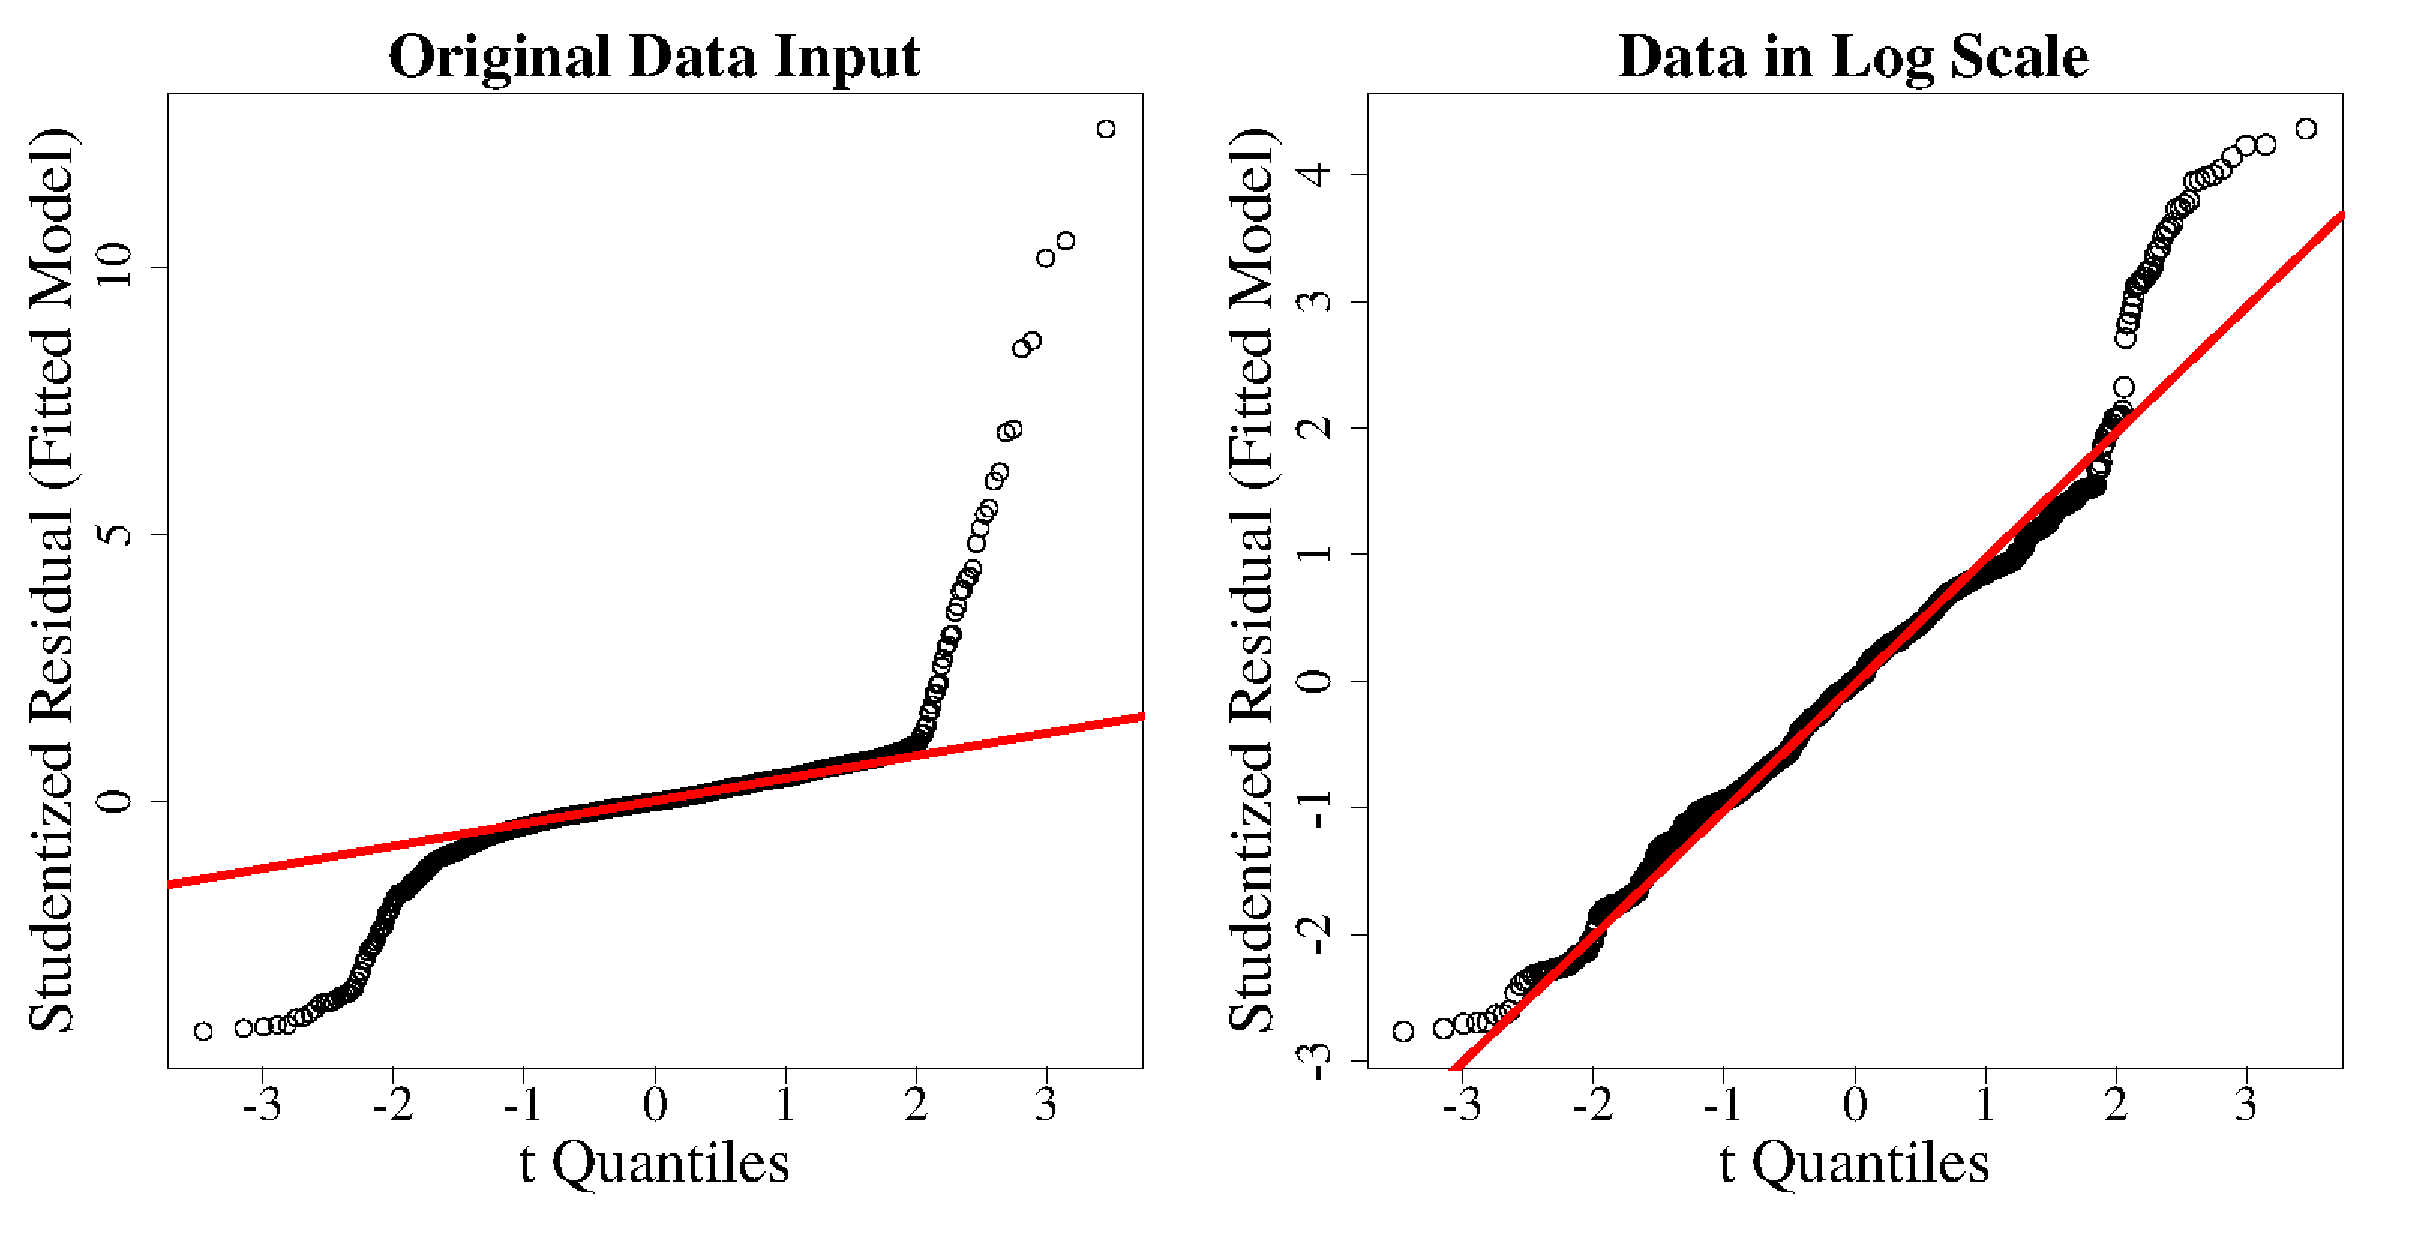
\includegraphics[scale=.3]{./images/QQplot.eps}
 \caption{Quantile-Quantile Analysis of the generated models}
 \label{fig:QQplot}
\end{figure}


\subsection{ML with extraction features}\label{ssec:methodExrtact}

In a machine learning process, the accuracy of the predictions depends on the quality of the pre-processing phase~\citep{Dasu:2003:EDM:861869}. In this section, we present a extraction features process to determine a set of parameters that permits predicting the running time of GPU applications in different contexts or scenarios. As it was mentioned above, we collected separately the set of events and metrics and the execution times of each application of Section~\ref{ssec:useCases} over all GPUs presented in Section~\ref{ssec:GPUTestbed}. 

To do these experiments, kernels of matrix addition, dot product, vector addition and sub-array maximum problem were used. The same number of samples than last section was used. All Rodinia applications were used. As before was mentioned, to limit the bias on the learning algorithms, we selected 100 random samples from the other applications. In total 16 kernels were used for these experiments. It was, this sampled data, that was used as dataset for the ML algorithms. 

We cleaned the collected information, dropping features with no variation among executions and without concordance among GPUs. Each cleaned sample of the dataset resulted in 85 kernel features plus 11 GPU architecture features, for a total of 96 features. We then performed a correlation analysis, followed by a clustering analysis to reduce the number of features (dimensionality reduction). 

We first transformed the data into a $log_2$ scale and, followed by a normalization, reducing the non-linearity effects~\citep{Barnes:2008:RAS} (line 2 and 3 of Algorithm~\ref{fig:methods}). To select a small number of application execution features to use with the ML algorithms, we performed correlation and clustering analyses over the data. We performed the correlation analysis using the Spearman Correlation Coefficient (SCC), since it captures relations and variations among features over different scales by using the rank values of the features. We evaluated the SCC for all features against the kernel execution times and applied a threshold of 0.75, keeping only the 21 features that had a SCC above it (line 4). These features are shown below:

\begin{algorithm}[htpb]
\SetAlgoLined
\KwResult{Prediction of the ML techniques}
\textbf{Input: Data sets}\;
ScaledData = scaleLog(Data sets)\;
NormalizedData = Normalize(ScaledData)\;
SCC = corr(NormalizedData, 0.75)\;
    \ForAll{No. Param in [5, 10]}{
    dendroG = hclust(corr(SCC))\;
    cutDendro = cutTree(dendroG, No. Param)\;
    features = variance(cutDendro)\;
        \ForAll{context in [GPUs, Kernels]}{
        \ForAll{ML in [LM, SVM, RF]}{
        trainingSet != features[context]\;
        testSet == features[context]\;
        
        Model = ML( trainingSet)\;
        output = predict(testSet)\;
        }
     }
 }
\caption{Algorithm of the methodological process done in this second approach} 
\label{fig:methods}
\end{algorithm}

\begin{lstlisting}[basicstyle=\small, numbers=none]
 [1] "elapsed_cycles_sm"                 
 [2] "gld_inst_32bit"                    
 [3] "gst_inst_32bit"                    
 [4] "inst_executed"                     
 [5] "inst_issued1"                      
 [6] "gld_request"                       
 [7] "gst_request"                       
 [8] "active_cycles"                     
 [9] "global_load_transactions"          
[10] "global_store_transactions"         
[11] "device_memory_read_transactions"   
[12] "l2_read_transactions"              
[13] "l2_write_transactions"             
[14] "issued_control.flow_instructions"  
[15] "executed_control.flow_instructions"
[16] "issued_load.store_instructions"    
[17] "executed_load.store_instructions"  
[18] "issue_slots"                       
[19] "control.flow_instructions"         
[20] "load.store_instructions"           
[21] "misc_instructions"  
\end{lstlisting}

To further reduce the features, we used a hierarchical clustering algorithm. We first create a similarity matrix over all features, using the Spearman correlation coefficient. This similarity matrix is the input for the clustering algorithm. This algorithm them performs the hierarchical clustering by first assigning each feature to its own cluster, and then proceeding iteratively, at each stage joining the two most similar clusters, continuing until there is just a single cluster, as shown in Figures~\ref{fig:Cuthclust:5} and \ref{fig:Cuthclust:10}, which present dendrograms built from 20 features. 

\begin{figure}[htbp]
    \centering
    \includegraphics[scale=.75]{./images/cluster-5.pdf}
    \caption{Dendrogram with 5 clusters to select 1 features from each one}
    \label{fig:Cuthclust:5}
\end{figure}

We can then select a number of clusters by cutting the tree at a certain height. For instance, in Figure~\ref{fig:Cuthclust:5}, the horizontal blue dashed line cuts the tree in a height that keeps 5 clusters and in Figure~\ref{fig:Cuthclust:5}, the horizontal blue dashed line cuts the tree in a height that keeps 10 clusters. Finally, we performed a variance analysis to select which feature correlates better with the kernel execution time. 

\begin{figure}[htbp]
    \centering
    \includegraphics[scale=.75]{./images/cluster-10.pdf}
    \caption{Dendrogram with 10 clusters to select 1 features from each one}
    \label{fig:Cuthclust:10}
\end{figure}

Regarding the GPU parameters, we performed a correlation analysis and experimented with different number of parameters. As, it was not possible to get a high Spearman  Correlation Coefficient with the GPU parameters, the parameters were taken considering the order of the SCC. In this way, we compared the GPU parameters against the kernel execution times and tested with different number of GPU parameters. GPU parameters were 11 and during the experiments we concluded that few GPU parameters captured the relations between hardware and applications.


\begin{lstlisting}[basicstyle=\small,numbers=none]
[1]  compute_capability
[2]  gpu_clock_rate
[3]  num_of_cores
[4]  num_of_sm
[5]  num_sp_per_sm
[6]  L2_size
[7]  bus
[8]  memory_clock
[9]  theoretical_flops
[10] bandwidth
[11] global_memory_size
\end{lstlisting}

In these experiments, we used three different machine learning methods: Linear Regression, Support Vector Machines and Random Forest. These machine learning techniques achieved a high precision in the predictions with the extracted features. Ensemble methods were also tested, but the additional computational complexity did not justify the small improvement in accuracy of the predictions. We evaluate the ML algorithms using sets of 5 and 10 features, and considered two experimental contexts:

\begin{enumerate}
\item GPUs: we evaluated if the ML algorithm could predict the execution time over a previously unseen GPU. We used a leave-one-out cross validation procedure, by selecting the samples from one GPU as a test set and using the samples from the other 8 GPUs as training set.

\item Kernels: in this case we predict the execution time of a previously unseen CUDA kernel. We used the same leave-one-out cross validation procedure, but now selecting the samples from a single kernel as a test set and using the samples from the other 15 kernels as training set.
\end{enumerate}




\section{Experimental Results}\label{sec:resultML}
\subsection{Results without extraction features}
% \todoRaph{You discussed only the procedure for the analytical model. You must do the same for the machine learning algorithms. You should include the number of repetitions used to obtain the training examples, the range of problem size values used, including the step size in the range, etc. The description must be as complete as possible. Also, what was the stop criteria in the laerning phase. Did you use a validation set?}

Figures~\ref{fig:Results-NCA-Fair} and ~\ref{fig:Results-RodiniaFair} shows a comparison between the accuracy of the Linear Regression (LR), Random Forest (RF) and SVM Regression (SVM) to predict execution times of each application on each target GPU. Figure  Each box plot represents accuracy per GPU, with each column representing a different technique and each line a different application. These figures show that we could reasonably predict the running time of 20 CUDA kernels over different GPUs belonging to 3 different architectures using machine learning techniques. 

% \todoRaph{Remember the reader that for each box you trained the machine learnign algorithm using the other GPUs. Also remember what you did with the AM}

% \todoRaph{Can't you just change the number of used threads in the analytical model equation??? Maybe this will solve the problem. I particularly prefer the analytical model over the machine learning, since it provides more information on the features of the model that results in performance predictions.} 


\begin{figure}[htpb]
    \centering
    \includegraphics[scale=1]{images/ResultTechniques-fair.pdf}
    \caption{Accuracy}
    \label{fig:Results-NCA-Fair}
\end{figure}

\begin{figure}[htpb]
    \centering
    \includegraphics[scale=1]{images/ResultTechniques-Rodinia-fair.pdf}
    \caption{Accuracy}
    \label{fig:Results-RodiniaFair}
\end{figure}

Table~\ref{tab:MAPE:NCA} and \ref{tab:MAPE:Rodinia} shows the comparison between both analytical model and machine learning approaches in terms of Mean Absolute Percentage Error (MAPE). This table shows that both analytical model and machine learning techniques obtained reasonable predictions for almost all cases. 

% \todoRaph{Why you do not show the MAPE results for the AM? Even if they are large, I do not see any problem in showing them.} 

The Analytical model presented MAPE around of 5\% for almost all the vector/matrix applications. This adjustment with this $\lambda$ parameters will give us reasonable prediction until certain circumstances, in others the analytical model always will need calibration. Machine learning techniques can do better predictions whether more samples from each class of CUDA kernels and better features are determined.

\begin{table}[htpb]
\centering
\scalebox{1}{
\small
\begin{tabular}{| c | c | c  |  c | c |} 
\midrule%inserts double horizontal lines
\multirow{2}{*}{\textbf{Apps}}&\multicolumn{4}{c|}{\textbf{MAPE ML Techniques}}\\\cline{2-5}
&\textbf{AM}&\textbf{LR}&\textbf{SVM}&\textbf{RF}\\\midrule
MMGU & 3.75$\pm$5.14&16.47$\pm$13.40&23.06$\pm$16.85&10.44$\pm$9.82\\ \midrule
MMGC & 6.70$\pm$2.07&15.53$\pm$11.28&15.23$\pm$5.76&10.02$\pm$7.21\\ \midrule
MMSU & 5.15$\pm$2.19&5.33$\pm$1.93&15.36$\pm$9.64&4.84$\pm$1.94\\ \midrule
MMSC & 3.46$\pm$2.11&14.83$\pm$10.22&20.28$\pm$14.23&8.53$\pm$3.02\\ \midrule
MAU & 8.00$\pm$3.20&69.51$\pm$51.77&19.90$\pm$14.73&37.92$\pm$23.57\\ \midrule
MAC & 6.50$\pm$4.08&12.65$\pm$2.77&18.94$\pm$7.71&10.74$\pm$3.80\\ \midrule
dotP & 4.54$\pm$2.94&3.30$\pm$1.42&15.90$\pm$8.41&4.57$\pm$1.25\\ \midrule
vAdd & 3.58$\pm$2.00&18.98$\pm$16.56&15.11$\pm$6.76&8.72$\pm$4.51\\ \midrule
MSA & 3.00$\pm$1.22&2.99$\pm$1.73&10.64$\pm$4.95&5.81$\pm$4.23\\ \midrule\end{tabular}
}
\caption{MAPE of the different techniques used}
\label{tab:MAPE:NCA} 
\end{table}

\begin{table}[htpb]
\centering
\scalebox{.85}{
\begin{tabular}{|r|c|c|c|c|}
\hline\hline
\textbf{Kernels/Techn.} &\textbf{AM}& \textbf{LR}&\textbf{SVM}&\textbf{RF}\\ \hline
                         
BCK-K1 & 3.53$\pm$1.25&108.61$\pm$215.21&17.66$\pm$21.44&31.58$\pm$27.87\\ \midrule
BCK-K2 & 4.86$\pm$3.33&26.00$\pm$30.54&25.98$\pm$34.53&128.20$\pm$261.96\\ \midrule
GAU-K1 & 31.53$\pm$3.85&27.36$\pm$26.88&14.19$\pm$3.16&18.98$\pm$14.67\\ \midrule
GAU-K2 & 78.31$\pm$4.58&20.94$\pm$6.09&14.55$\pm$7.63&18.42$\pm$7.71\\ \midrule
HTW & 13.09$\pm$1.72&25.49$\pm$31.46&25.38$\pm$21.88&26.62$\pm$30.17\\ \midrule
HOT & 3.86$\pm$2.18&44.55$\pm$30.51&28.60$\pm$20.98&118.72$\pm$202.31\\ \midrule
LUD-K1 & - &3902028.92$\pm$8725176.99&11.20$\pm$11.63&11.03$\pm$7.73\\ \midrule
LUD-K2 & - &35.61$\pm$19.77&25.97$\pm$17.41&54.64$\pm$78.61\\ \midrule
LUD-K3 & - &46.53$\pm$34.59&18.57$\pm$10.46&43.78$\pm$33.70\\ \midrule
NDL-K1 & - &17.65$\pm$7.77&13.08$\pm$7.25&13.90$\pm$3.79\\ \midrule
NDL-K2 & - &15.18$\pm$2.86&10.82$\pm$3.85&13.40$\pm$3.49\\ \midrule
\end{tabular}}
\caption{MAPE of the prediction of the second context (in \%).}
\label{tab:MAPE:Rodinia}
\end{table}

\subsection{Results with extraction features}
We first performed the process of feature extraction. After applying the correlation and hierarchical clustering, we selected the 10 features below. The first 5 features are used in the experiments with 5 features, and the complete set is used for the experiments with 10 features.

\begin{lstlisting}[basicstyle=\small,numbers=none]
 elapsed_cycles_sm"                 
 [2] "gld_request"                       
 [3] "gst_request"   
 [4] "executed_control.flow_instructions"
 [5] "device_memory_read_transactions"                         
 [6] "active_cycles"                     
 [7] "global_store_transactions"         
 [8] "gst_inst_32bit"                    
 [9] "executed_load.store_instructions"  
[10] "misc_instructions"  
\end{lstlisting}

As it was mentioned in the last section we used two metrics, accuracy and Mean Absolute Percentage Error (MAPE) of the predictions of each machine learning algorithm. The accuracy is the ratio $t_k/t_m$, between the predicted times $t_k$ and the measured times $t_m$. MAPE is computed using equation~\ref{ec:MAPE}.

We evaluate the MAPE for each learning algorithm, linear regression (LR), support vector machine (SVM) and random forest (RF), when using 2 GPU parameters (number of cores and amount of L2 cache), when considering either 5 or 10 application features. We justify the selection of these 2 GPU parameters later in this section.

Table~\ref{tab:MAPE:Contex1} shows the MAPE for the ML algorithms for the first scenario, where we predict the execution time over a previously unseen GPU. %Blue and red cells represent the best and worst MAPE for each predicted GPU, respectively. Linear Regression obtained the best MAPE in 5 different GPUs, while Random Forests was better for the other 3 GPUs. Both LR and SVM benefited from using 10 features, while for RF it was better to use only 5 features. But overall, using LR with 5 features provided reasonably good predictions using a simple ML procedure and very few features. 



\begin{table}[htpb]
\centering
\scalebox{1}{
\small
\begin{tabular}{| c | c | c  |  c | c | c  |  c | } 
\midrule%inserts double horizontal lines
\multirow{2}{*}{\textbf{GPUs}}&\multicolumn{6}{c|}{\textbf{MAPE ML Techniques per Number of Features}}\\\cline{2-7}
&\multicolumn{2}{c|}{\textbf{LR}}&\multicolumn{2}{c|}{\textbf{RF}}&\multicolumn{2}{c|}{\textbf{SVM}}\\\midrule
& \textbf{5}&\textbf{10}& \textbf{5}&\textbf{10}& \textbf{5}&\textbf{10}\\\midrule
GTX-680 & 1.75&1.63&2.70&2.68&1.95&1.59\\ \midrule
Tesla-K40 & 1.24&1.10&0.73&0.69&1.63&1.46\\ \midrule
Tesla-K20 & 1.40&1.13&1.48&1.41&1.74&1.51\\ \midrule
Titan & 1.29&1.21&1.22&0.97&1.61&1.53\\ \midrule
Quadro & 2.62&2.24&3.23&3.16&2.89&2.34\\ \midrule
TitanX & 2.52&2.79&2.36&2.07&2.79&2.93\\ \midrule
GTX-970 & 2.00&2.41&2.93&2.88&2.26&3.10\\ \midrule
GTX-980 & 1.74&1.54&1.97&1.68&1.97&1.77\\ \midrule
Tesla-P100 & 3.71&4.49&7.89&8.36&4.06&4.23\\ \midrule
\end{tabular}
}
\caption{MAPE of the prediction of the first context (in \%). }
\label{tab:MAPE:Contex1} 
\end{table}

Table~\ref{tab:MAPE:Contex2} shows the MAPE of the ML algorithms when predicting the execution time of a previously unseen application. LM and SVM with 5 features obtained the best average MAPEs and seem appropriate choices for predicting the execution times. Although RF obtained the best MAPE for 6 kernels, it obtained poor MAPEs for some kernels, resulting in larger average MAPEs. Considering the results from both contexts (Tables~\ref{tab:context1} and Table~\ref{tab:context2}), it seems that using LR with 5 parameters is a better overall choice.


\begin{table}[htpb]
\centering
\scalebox{1}{
\small
\begin{tabular}{| c | c | c  |  c | c | c  |  c |} 
\midrule%inserts double horizontal lines
\multirow{2}{*}{\textbf{Kernels}}&\multicolumn{6}{c|}{\textbf{MAPE ML Techniques per Number of Features}}\\\cline{2-7}
&\multicolumn{2}{c|}{\textbf{LR}}&\multicolumn{2}{c|}{\textbf{RF}}&\multicolumn{2}{c|}{\textbf{SVM}}\\\midrule
& \textbf{5}&\textbf{10}& \textbf{5}&\textbf{10}& \textbf{5}&\textbf{10}\\\midrule
BCK-K1&2.07&2.11&1.64&1.88&2.69&1.78\\ \midrule
BCK-K2&2.87&2.62&3.25&2.97&2.46&2.69\\ \midrule
GAU-K1&3.98&4.60&3.36&3.59&9.49&9.29\\ \midrule
GAU-K2&1.50&1.80&9.36&6.61&8.02&11.30\\ \midrule
HTW&3.78&2.86&6.51&5.43&4.52&4.74\\ \midrule
HOT&2.56&2.40&2.57&2.35&10.12&8.01\\ \midrule
LUD-K1&4.02&4.18&2.13&4.19&15.72&15.36\\ \midrule
LUD-K2&1.88&2.09&2.16&3.19&2.28&2.42\\ \midrule
LUD-K3&0.98&1.17&1.83&1.93&1.48&1.44\\ \midrule
NDL-K1&1.14&1.18&0.54&0.49&1.65&1.93\\ \midrule
NDL-K2&1.03&1.01&0.47&0.50&1.59&1.91\\ \midrule
MAU&2.18&3.87&13.22&10.73&13.37&14.38\\ \midrule
MAC&1.38&1.37&1.91&2.10&2.07&1.72\\ \midrule
dotP&2.47&10.88&8.42&6.11&9.38&12.44\\ \midrule
vAdd&2.93&4.25&3.95&2.57&2.54&2.96\\ \midrule
MSA&18.65&12.14&41.22&39.03&48.19&39.53\\ \midrule


\end{tabular}
}
\caption{MAPE of the prediction of the second context (in \%). }
\label{tab:MAPE:Contex2} 
\end{table}

For each context, we also tested the number of GPU parameters (features) to use. Figure~\ref{fig:GPUParam} shows the average MAPE of the linear regression model with different numbers of GPU parameters in both contexts. Figure~\ref{fig:GPUParam-RF} show the average MAPE of the random forest with different numbers of GPU parameters in both contexts. We can see that 2 parameters provided the smaller error for 5 application features. For 10 features, including more parameters decreased only slightly the average MAPE for linear regression model, increased for random forests. Consequently, we decided to use 2 GPU parameters in the experiments. The evaluated GPU parameters are shown below, ordered from higher to lower Spearman coefficient against execution times.

\begin{lstlisting}[basicstyle=\small, numbers=left, stepnumber=1]
L2
num_cores_sm
memory_clock
compute_version
theoretical_flops
max_clock_rate
\end{lstlisting}

\begin{figure}[htpb]
    \centering
    \includegraphics[scale=.75]{./images/parameters.pdf}
    \caption{Best number of GPU parameters in each one of the contexts for Linear Regression}
    \label{fig:GPUParam}
\end{figure}

 
\begin{figure}[htpb]
    \centering
    \includegraphics[scale=.75]{./images/parameters-RF.pdf}
    \caption{Best number of GPU parameters in each one of the contexts for Random Forests}
    \label{fig:GPUParam-RF}
\end{figure}


Figures~\ref{fig:Results-contex1},  \ref{fig:Results:context2:NCA} and \ref{fig:Results:context2:Rodinia} show box plots of the accuracies of individual samples for the first scenario of GPUs and second scenario of vector matrix CUDA kernels and second scenario of Rodinia CUDA kernels, respectively. The boxes represent the median and the upper and lower first quartiles, with whiskers representing the maximum and minimum possible errors. Outliers are marked as individual points.

\begin{figure}[htpb]
    \centering
    \includegraphics[scale=.5]{images/ResultTechniques-Context1.pdf}
    \caption{Accuracy ($t_k/t_m$) of the first scenario with GPUs of 3 different architectures}
    \label{fig:Results-contex1}
\end{figure}

\begin{figure}[htpb]
    \centering
    \includegraphics[scale=.65]{images/ResultTechniques-Context2-NCA.pdf}
    \caption{Accuracy of the 5 vector/matrix CUDA kernels used in the second scenarios}
    \label{fig:Results:context2:NCA}
\end{figure}

\begin{figure}[htpb]
    \centering
    \includegraphics[scale=.5]{images/ResultTechniques-Context2-Rodinia.pdf}
    \caption{Accuracy of the second scenarios of the Rodinia CUDA kernels}
    \label{fig:Results:context2:Rodinia}
\end{figure}

Overall, the predictions for the first context (Figure~\ref{fig:Results-contex1}) was good, with the most samples with a accuracy between 0.9 and 1.1. For the second context (Figure~\ref{fig:Results:context2:NCA} and ~\ref{fig:Results:context2:Rodinia}) the predictions were less accurate for some kernels, but for the SVM and linear regression they were still mostly between 0.85 and 1.15. SVM and LR obtained similar accuracies because we used a linear kernel for SVMs, since it provided than using nonlinear kernels, such as polynomial, Gaussian (RBF) and sigmoid. For Random Forests, we set the number of trees to $50$, and the number of predictor candidates at each split to $3$, as these values resulted in better predictions and faster executions. 


\section{Related Works}\label{sec:relatedWorksML}
Some authors have focused their works on performance prediction of applications using machine learning~\citep{Jiangtian:2009, Ozisikyilmaz:2008, Singh:2007:PPA, Ipek:2005:APP,Matsunaga:2010}. The main learning algorithms that they used were statistical methods, Neural Networks, Support Vector Machines, and Random Forest.

In  recent  years,  studies on GPU performance using different statistical and machine learning approaches have appeared. ~\cite{Baldini:2014} showed that machine learning can predict GPU speedup from OpenMP applications. They used K-nearest neighbor and SVM as classifier to know the performance of these applications over different GPUs. 

In  recent  years, studies on comparison of GPU performance using analytical modeling, statistical analysis and machine learning approaches have appeared. ~\cite{Madougou:2016} presented a comparison between different GPGPU performance modeling tools, they compare between analytical model, statistical approaches, quantitative methods and compiler-based methods. In this works, authors concluded that the available GPU performance modeling solutions are very sensitive to applications and platform changes, and require
significant efforts for tuning and calibration when new analyses are required.

~\cite{Baldini:2014} showed that machine learning can predict GPU speedup of OpenCL applications from OpenMP applications. They used K-nearest neighbor and SVM as classifier to know the performance of these applications over different GPUs. They showed that a small set of easily-obtainable features can predict the magnitude of GPU speedups on two different high-end GPUs, with accuracies varying between 77\% and 90\%, depending on the prediction mechanism and scenario.

~\cite{Kerr:2012:Eiger} developed a methodology for the systematic construction of performance models of heterogeneous processors. They developed a framework, named Eiger, that implements their methodology. This methodology is comprised of experimental data acquisition and database construction, a series of data analysis passes over the database, and model selection and construction. They collected data from a simulator of GPU application named Ocelot, they defined a functional simulator~\cite{kerr2009characterization} for specific Nvidia PTX code. 

~\cite{Singh:2007:PPA} were one of the firsts authors to compare performance predictions of parallel computing models~\cite{Juurlink:1998}, comparing BSP, E-BSP and BPRAM over different parallel platform. Some authors have also focused their work in performance prediction of parallel applications using machine learning. All this work is about parallel applications executed over CPUs and not GPU applications.

~\cite{Greathouse:2015:GPGPUML} described a GPU performance and power estimation model, using K-means to create sets of scaling behaviors representative of the training kernels and neural networks that map kernels to clusters, with experiments using OpenCL applications over AMD GPUs. ~\cite{Karami:2013} proposed a statistical performance prediction model for OpenCL kernels on NVIDIA GPUs using a regression model for prediction and principle component analysis for extracting features of higher weights, thus reducing model complexity while preserving accuracy. 

~\cite{Hayashi:2015:MPH} presented  a statistical approach on  the  performance and power consumption of an ATI GPU~\cite{Zhang:2011}, using Random Forest due to its useful interpretation tools. Hayashi et al. constructed a prediction model that estimates the execution time of parallel applications based on a binary prediction model with Support Vector Machines for runtime CPU/GPU selection. 
%Kerr et al. developed Eiger~\cite{Kerr:2012:Eiger}, which is a framework for automated  statistical approaches for modeling program behaviors on diverse GPU architectures. They used various approaches, among them principal component analysis, clustering techniques, and regression analysis. %Madougou et al. presented a comparison between different GPGPU performance modeling tools~\cite{Madougou2016}, they compare between analytical model, statistical approaches, quantitative methods and compiler-based methods. 

~\cite{meswani:IPDPSW:2012} predicted the performance of HPC applications on hardware accelerators such as FPGA and GPU from applications running on CPU. This was done by identifying common compute patterns or idioms, then developing a framework to model the predicted speedup when the application is run on GPU or FPGA using these idioms. ~\cite{Ipek:2005:APP} trained multilayer neural networks to predict different performance aspects of parallel applications using input data from executing applications multiple times on the target platform.

In this work, we compare three different machine learning techniques to predict kernel execution times over NVIDIA GPUs. Moreover, we also perform a comparison with a BSP-based analytical model to verify when each approach is advantageous.




% In this work, we compare three different machine learning techniques to predict kernel execution times over NVIDIA GPUs. We also perform a comparison with a BSP-based analytical model to verify when each approach is advantageous. Although some works have compared analytical models, statistical approaches and quantitative methods, to the best of our knowledge this is the first work that compares analytical model to machine learning techniques to predict running times of GPU applications. Moreover, it offers a comparison between different machine learning techniques.

